\section{Introduction}
\subsection{Research problem}
Fireworks dispersal may concentrate thousands of passengers within a short time at Beimen and nearby stations. For operations planning, three distinct quantities must not be conflated: hourly tap-in demand, the minute at which a passenger reaches a platform, and the available space on a passing train. A plausible hourly forecast can still yield an inadequate timetable when its largest hour is underpredicted or when arrivals cluster within that hour. Conversely, a timetable that reduces simulated waiting may incur additional cash expenditure. This study therefore follows the complete chain from data to an explicitly limited timetable decision.

The research questions are:
\begin{enumerate}[leftmargin=2em]
\item How well does the frozen event-day hourly forecast perform relative to transparent rules that use the same chronological cutoffs and evaluation events?
\item How sensitive is platform waiting to unobserved within-hour arrivals and train space?
\item Relative to a reference timetable, what operating-expenditure and waiting-time trade-offs arise when Green-line services may be added, cancelled or retimed?
\end{enumerate}
The first two questions are statistical and simulation questions; the third is a finite-candidate decision comparison. The paper makes no causal claim that a particular festival attribute independently creates a stated number of metro entries, and it does not infer a real-time train-dispatch order.

\subsection{Study contributions and scope}
The contribution is a reproducible, auditable sequence rather than a new forecasting algorithm. First, all models and three simple benchmarks share forward-year test folds. Second, the information available at the proposed day-before forecast time is separated from retrospective measurements. Third, hourly predictions feed explicit minute-arrival and capacity scenarios rather than an unlabelled queueing calculation. Fourth, the latest timetable experiment keeps the original Green-line service as a comparator and reports cash expenditure separately from monetized waiting. A companion appendix states mathematical results and their assumptions. Figure~\ref{fig:workflow} summarizes the sequence; its editable source is \texttt{workflow\_en.mmd}.
\begin{figure}[htbp]\centering
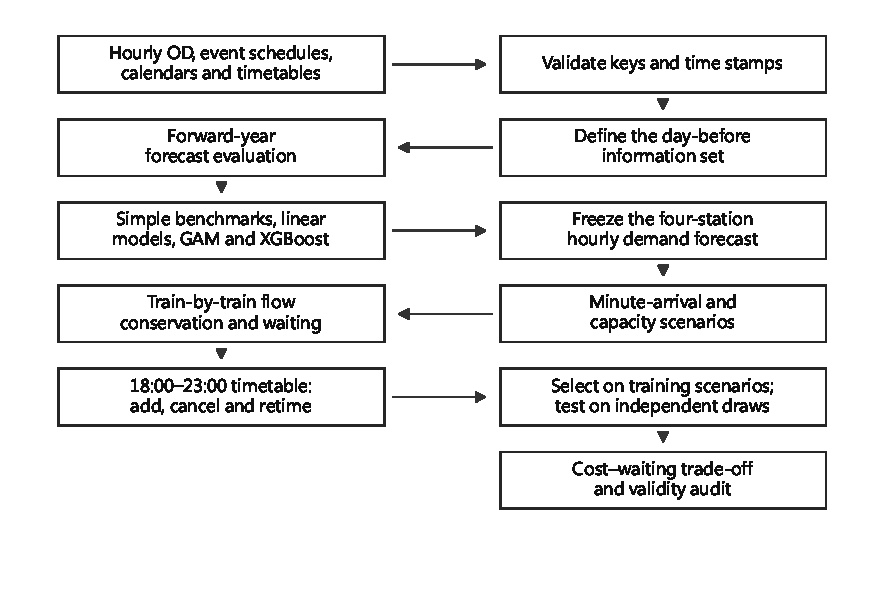
\includegraphics[width=.94\linewidth]{workflow_en.pdf}
\caption{Research workflow. Boxes distinguish forecasting, conditional queue simulation, and timetable evaluation. The diagram is a design description, not evidence that every input is prospectively available.}
\label{fig:workflow}
\end{figure}

\section{Related literature and methodological rationale}
Ridge regression shrinks coefficients when regressors are strongly correlated, while the Lasso can set coefficients to zero \cite{ridge,lasso}. These properties justify including both as interpretable linear comparators; they do not imply that either must predict event peaks well. Generalized additive models (GAMs) offer smooth nonlinear partial effects while retaining additive interpretability \cite{gam,pspline}. XGBoost can represent threshold and interaction patterns with regularized boosted trees \cite{xgb}. We therefore compare model families with distinct inductive biases, rather than claiming that more complex models are intrinsically preferable.

Temporal evaluation must preserve chronology and event grouping. Forward-origin validation motivates the annual splits \cite{fpp}. Nevertheless, repeated inspection of the same small set of final events can produce selection bias even if individual fitting steps are chronologically correct \cite{cawley}. This distinction matters here because the fourfold dispersal training weight was retained after comparisons involving the nine events.

For waiting, Little's steady-state relation is informative but not a license to treat a fireworks surge as a stationary M/M/$c$ queue \cite{little}. We use a finite-horizon, train-arrival batch-service representation and derive its passenger-minute accounting directly. Rail-corridor research has considered passenger waiting and operating cost jointly \cite{pan}; our cost function and candidate search are specific to this project and are not presented as a reproduction of that paper's model. These references support the methodological families, while the numerical settings below remain project assumptions.

\section{Data and study design}
\subsection{Observation units and provenance}
The outcome is the number of tap-ins at station $s$ during source hour $h$ on held event date $d$, denoted $Y_{dsh}$. The four stations are Beimen, Daqiaotou, Shuanglian and Minquan West Road; the hours are 18:00--23:00. Twenty-one events yield $21\times4\times6=504$ rows. Rows from one event share many determinants and are not 504 independent events. The main forecast evaluation is the nine Beimen events from 2024, 2025 and 2026, hence $9\times6=54$ rows.

The primary source is Taipei Metro's hourly origin--destination (OD) data \cite{metrodata}. In the source convention, an OD record associated with a destination such as Beimen retains its \emph{origin} time bin; aggregating such records by destination is not a direct hourly exit-gate count. Published calendars and pre-announced event programs supply candidate date and dispersal features. Official timetable PDFs and adjacent-station travel times supply an operational reference, but the available timetable edition is not confirmed to be the actual historical timetable of every event. Observed weather from the Central Weather Administration, annual budget records, social posts and search interest provide contextual or exploratory information; observed weather and annual expenditure are not inserted into the frozen day-before demand model.

\begin{table}[htbp]\centering\small
\caption{Data layers, units, and their analytical roles.}
\label{tab:data}
\begin{tabularx}{\linewidth}{p{32mm}p{42mm}X}\toprule
Layer & Native unit & Role and qualification\\\midrule
Metro OD & origin station, destination station, source hour & Hourly outcome and background flow; historical release dates remain incompletely audited.\\
Event and calendar & event date, announced program, weekday/holiday & Scheduled dispersal overlap and date descriptors; actual ending time is excluded from the day-before model.\\
Ordinary-day reference & station, source hour, selected comparator dates & Retrospective 56-day station-hour baseline; both a model feature and a standalone rule in this paper.\\
Train timetable & service, direction, station, time & Reference and candidate service schedules; not a certified record of every historical event-day dispatch.\\
Train loading & inferred passengers per service & Simulated from OD and routing; matched historical measured train loads are unavailable.\\
Weather, publicity, finance & observation time, post, or fiscal year & Contextual/sensitivity information; an annual publicity total is not a per-event amount.\\\bottomrule
\end{tabularx}
\end{table}

\subsection{The ordinary-day reference and the information frontier}
The archived feature \texttt{retrospective\_baseline\_56d}, here written $B_{dsh}$, averages at most four nearest eligible comparator days selected among the preceding eight same weekdays. Selection excludes listed event days and incomplete 18:00--24:00 records and requires matching holiday/makeup-workday classification and calendar note; at least two days are required for the original event-level eligibility rule. It is \emph{not} an average over every day in a 56-day block. An independent hourly replay stored at \texttt{.local/research\_review/2026-10-07-independent-review/independent\_hourly\_baselines.csv} reproduces all 504 archived baseline values to numerical tolerance (maximum absolute difference $2.84\times10^{-14}$). This reconciles the calculation, not the historical public availability of each input. The earlier four-week/eight-week event-versus-normal analysis is a separate descriptive comparison, not a forecasting score on the same nine-event panel.

Let $t_0(d)$ be the planned forecast issue time on the day before event $d$. A true prospective input requires
\begin{equation}
\operatorname{available\_at}(X_{dsh,j})\leq t_0(d)
\quad\text{for every input column }j.
\label{eq:frontier}
\end{equation}
Calendar fields can be computed before $d$; scheduled ending times can be used only if their announcement preceded $t_0(d)$. Actual event end times, observed weather and post-event social volume do not meet this rule. The annual holdout experiments follow a day-before \emph{design}, but the release timestamps of all historical OD and calendar snapshots were not fully reconstructed. Thus the work is a retrospective as-of sensitivity study, not a verified deployable D$-1$ forecast.

\subsection{Data processing, missingness, and storage}
The analysis key is $(d,s,h)$. Numeric parsing, duplicate checks, six-hour coverage checks and station labels precede estimation. Optional fields have missingness indicators and training-fold-only imputation; missing is not silently recoded to observed zero. Continuous features are standardized using training-fold moments, and categories and interaction columns are learned from that fold. Exact linear dependencies are removed without consulting outcomes. The OD preparation uses DuckDB and Parquet for large scans; relational MySQL tables store activities, weather observations, station metadata and annual finance with keys. This storage division affects reproducibility and query cost but not the statistical estimand. Raw/private snapshots and model artifacts are excluded from the public repository, so the manuscript gives both source identifiers and a private-input reproduction requirement.
